% OK!
\chapter{Développement durable}

À l'heure où la France s'inquiète de l'impact écologiques sur la planète des climatiseurs pour refroidir nos pièces durant les fortes chaleurs, ce problème ne semble pas être au cœur des préoccupations par UTP.

Les températures extérieures étant très élevées en Malaisie, tous les bâtiments (gares, restaurants, hôtels, etc.) et les voitures sont équipés de climatiseurs. Cependant, le réglage de ces derniers provoque des températures intérieures souvent bien trop froides ($\approx 20^{\circ}C$) et nous oblige à porter des vêtements chauds et longs à l'intérieur des bâtiments malgré la température extérieure dépassant largement les $30^{\circ}C$ l'ensemble de  notre séjour.

\begin{figure}[h]
  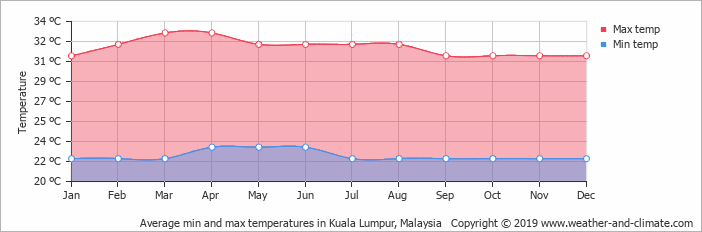
\includegraphics[width=1\linewidth]{content/imgs/temp.png}
  \caption{Températures moyennes minimales et maximales en Malaisie, dans la capitale}
  \label{fig:climate}
\end{figure}

Malgré l'usage excessif des climatiseurs, les bâtiments récents de l'université ne sont pas dotés d'une isolation thermique comparable aux bâtiments récents de France. Pour ne prendre qu'un exemple, je travaillais dans la bibliothèque universitaire, cette dernière possède une immense façade vitrée bordée de portes, elles aussi vitrées, laissant la fraîcheur du bâtiment se faire ressentir sur plusieurs mètres à l'extérieur. De plus, les climatiseurs des laboratoires de l'université restent la plupart du temps allumés toute la journée malgré l'absence de personne dans ces pièces climatisées, et avec en plus les portes ouvertes (qui donnent directement sur l'extérieur).

D'après le site de l'université \cite{utp_gender}, une attention particulière est mise en œuvre pour favoriser la diversité des genres au sein de l'université, que ce soit au niveau des étudiants, des employés ou du personnel pédagogique.
